\documentclass[conference]{IEEEtran}
% Some/most Computer Society conferences require the compsoc mode option,
% but others may want the standard conference format.
%
% If IEEEtran.cls has not been installed into the LaTeX system files,
% manually specify the path to it like:
% \documentclass[conference,compsoc]{../sty/IEEEtran}


% Some very useful LaTeX packages include:
% (uncomment the ones you want to load)


% *** MISC UTILITY PACKAGES ***
%
%\usepackage{ifpdf}
% Heiko Oberdiek's ifpdf.sty is very useful if you need conditional
% compilation based on whether the output is pdf or dvi.
% usage:
% \ifpdf
%   % pdf code
% \else
%   % dvi code
% \fi
% The latest version of ifpdf.sty can be obtained from:
% http://www.ctan.org/pkg/ifpdf
% Also, note that IEEEtran.cls V1.7 and later provides a builtin
% \ifCLASSINFOpdf conditional that works the same way.
% When switching from latex to pdflatex and vice-versa, the compiler may
% have to be run twice to clear warning/error messages.

% *** CITATION PACKAGES ***
%
\ifCLASSOPTIONcompsoc
  % IEEE Computer Society needs nocompress option
  % requires cite.sty v4.0 or later (November 2003)
  \usepackage[nocompress]{cite}
\else
  % normal IEEE
  \usepackage{cite}
\fi
% cite.sty was written by Donald Arseneau
% V1.6 and later of IEEEtran pre-defines the format of the cite.sty package
% \cite{} output to follow that of the IEEE. Loading the cite package will
% result in citation numbers being automatically sorted and properly
% "compressed/ranged". e.g., [1], [9], [2], [7], [5], [6] without using
% cite.sty will become [1], [2], [5]--[7], [9] using cite.sty. cite.sty's
% \cite will automatically add leading space, if needed. Use cite.sty's
% noadjust option (cite.sty V3.8 and later) if you want to turn this off
% such as if a citation ever needs to be enclosed in parenthesis.
% cite.sty is already installed on most LaTeX systems. Be sure and use
% version 5.0 (2009-03-20) and later if using hyperref.sty.
% The latest version can be obtained at:
% http://www.ctan.org/pkg/cite
% The documentation is contained in the cite.sty file itself.
%
% Note that some packages require special options to format as the Computer
% Society requires. In particular, Computer Society  papers do not use
% compressed citation ranges as is done in typical IEEE papers
% (e.g., [1]-[4]). Instead, they list every citation separately in order
% (e.g., [1], [2], [3], [4]). To get the latter we need to load the cite
% package with the nocompress option which is supported by cite.sty v4.0
% and later.

% *** GRAPHICS RELATED PACKAGES ***
%
\ifCLASSINFOpdf
  % \usepackage[pdftex]{graphicx}
  % declare the path(s) where your graphic files are
  % \graphicspath{{../pdf/}{../jpeg/}}
  % and their extensions so you won't have to specify these with
  % every instance of \includegraphics
  % \DeclareGraphicsExtensions{.pdf,.jpeg,.png}
\else
  % or other class option (dvipsone, dvipdf, if not using dvips). graphicx
  % will default to the driver specified in the system graphics.cfg if no
  % driver is specified.
  % \usepackage[dvips]{graphicx}
  % declare the path(s) where your graphic files are
  % \graphicspath{{../eps/}}
  % and their extensions so you won't have to specify these with
  % every instance of \includegraphics
  % \DeclareGraphicsExtensions{.eps}
\fi
% graphicx was written by David Carlisle and Sebastian Rahtz. It is
% required if you want graphics, photos, etc. graphicx.sty is already
% installed on most LaTeX systems. The latest version and documentation
% can be obtained at: 
% http://www.ctan.org/pkg/graphicx
% Another good source of documentation is "Using Imported Graphics in
% LaTeX2e" by Keith Reckdahl which can be found at:
% http://www.ctan.org/pkg/epslatex
%
% latex, and pdflatex in dvi mode, support graphics in encapsulated
% postscript (.eps) format. pdflatex in pdf mode supports graphics
% in .pdf, .jpeg, .png and .mps (metapost) formats. Users should ensure
% that all non-photo figures use a vector format (.eps, .pdf, .mps) and
% not a bitmapped formats (.jpeg, .png). The IEEE frowns on bitmapped formats
% which can result in "jaggedy"/blurry rendering of lines and letters as
% well as large increases in file sizes.
%
% You can find documentation about the pdfTeX application at:
% http://www.tug.org/applications/pdftex

% *** MATH PACKAGES ***
%
%\usepackage{amsmath}
% A popular package from the American Mathematical Society that provides
% many useful and powerful commands for dealing with mathematics.
%
% Note that the amsmath package sets \interdisplaylinepenalty to 10000
% thus preventing page breaks from occurring within multiline equations. Use:
%\interdisplaylinepenalty=2500
% after loading amsmath to restore such page breaks as IEEEtran.cls normally
% does. amsmath.sty is already installed on most LaTeX systems. The latest
% version and documentation can be obtained at:
% http://www.ctan.org/pkg/amsmath

% *** SPECIALIZED LIST PACKAGES ***
%
%\usepackage{algorithmic}
% algorithmic.sty was written by Peter Williams and Rogerio Brito.
% This package provides an algorithmic environment fo describing algorithms.
% You can use the algorithmic environment in-text or within a figure
% environment to provide for a floating algorithm. Do NOT use the algorithm
% floating environment provided by algorithm.sty (by the same authors) or
% algorithm2e.sty (by Christophe Fiorio) as the IEEE does not use dedicated
% algorithm float types and packages that provide these will not provide
% correct IEEE style captions. The latest version and documentation of
% algorithmic.sty can be obtained at:
% http://www.ctan.org/pkg/algorithms
% Also of interest may be the (relatively newer and more customizable)
% algorithmicx.sty package by Szasz Janos:
% http://www.ctan.org/pkg/algorithmicx

% *** ALIGNMENT PACKAGES ***
%
%\usepackage{array}
% Frank Mittelbach's and David Carlisle's array.sty patches and improves
% the standard LaTeX2e array and tabular environments to provide better
% appearance and additional user controls. As the default LaTeX2e table
% generation code is lacking to the point of almost being broken with
% respect to the quality of the end results, all users are strongly
% advised to use an enhanced (at the very least that provided by array.sty)
% set of table tools. array.sty is already installed on most systems. The
% latest version and documentation can be obtained at:
% http://www.ctan.org/pkg/array

% IEEEtran contains the IEEEeqnarray family of commands that can be used to
% generate multiline equations as well as matrices, tables, etc., of high
% quality.

% *** SUBFIGURE PACKAGES ***
%\ifCLASSOPTIONcompsoc
%  \usepackage[caption=false,font=footnotesize,labelfont=sf,textfont=sf]{subfig}
%\else
%  \usepackage[caption=false,font=footnotesize]{subfig}
%\fi
% subfig.sty, written by Steven Douglas Cochran, is the modern replacement
% for subfigure.sty, the latter of which is no longer maintained and is
% incompatible with some LaTeX packages including fixltx2e. However,
% subfig.sty requires and automatically loads Axel Sommerfeldt's caption.sty
% which will override IEEEtran.cls' handling of captions and this will result
% in non-IEEE style figure/table captions. To prevent this problem, be sure
% and invoke subfig.sty's "caption=false" package option (available since
% subfig.sty version 1.3, 2005/06/28) as this is will preserve IEEEtran.cls
% handling of captions.
% Note that the Computer Society format requires a sans serif font rather
% than the serif font used in traditional IEEE formatting and thus the need
% to invoke different subfig.sty package options depending on whether
% compsoc mode has been enabled.
%
% The latest version and documentation of subfig.sty can be obtained at:
% http://www.ctan.org/pkg/subfig

% *** FLOAT PACKAGES ***
%
%\usepackage{fixltx2e}
% fixltx2e, the successor to the earlier fix2col.sty, was written by
% Frank Mittelbach and David Carlisle. This package corrects a few problems
% in the LaTeX2e kernel, the most notable of which is that in current
% LaTeX2e releases, the ordering of single and double column floats is not
% guaranteed to be preserved. Thus, an unpatched LaTeX2e can allow a
% single column figure to be placed prior to an earlier double column
% figure.
% Be aware that LaTeX2e kernels dated 2015 and later have fixltx2e.sty's
% corrections already built into the system in which case a warning will
% be issued if an attempt is made to load fixltx2e.sty as it is no longer
% needed.
% The latest version and documentation can be found at:
% http://www.ctan.org/pkg/fixltx2e


%\usepackage{stfloats}
% stfloats.sty was written by Sigitas Tolusis. This package gives LaTeX2e
% the ability to do double column floats at the bottom of the page as well
% as the top. (e.g., "\begin{figure*}[!b]" is not normally possible in
% LaTeX2e). It also provides a command:
%\fnbelowfloat
% to enable the placement of footnotes below bottom floats (the standard
% LaTeX2e kernel puts them above bottom floats). This is an invasive package
% which rewrites many portions of the LaTeX2e float routines. It may not work
% with other packages that modify the LaTeX2e float routines. The latest
% version and documentation can be obtained at:
% http://www.ctan.org/pkg/stfloats
% Do not use the stfloats baselinefloat ability as the IEEE does not allow
% \baselineskip to stretch. Authors submitting work to the IEEE should note
% that the IEEE rarely uses double column equations and that authors should try
% to avoid such use. Do not be tempted to use the cuted.sty or midfloat.sty
% packages (also by Sigitas Tolusis) as the IEEE does not format its papers in
% such ways.
% Do not attempt to use stfloats with fixltx2e as they are incompatible.
% Instead, use Morten Hogholm'a dblfloatfix which combines the features
% of both fixltx2e and stfloats:
%
% \usepackage{dblfloatfix}
% The latest version can be found at:
% http://www.ctan.org/pkg/dblfloatfix

% *** PDF, URL AND HYPERLINK PACKAGES ***
%
%\usepackage{url}
% url.sty was written by Donald Arseneau. It provides better support for
% handling and breaking URLs. url.sty is already installed on most LaTeX
% systems. The latest version and documentation can be obtained at:
% http://www.ctan.org/pkg/url
% Basically, \url{my_url_here}.

% *** Do not adjust lengths that control margins, column widths, etc. ***
% *** Do not use packages that alter fonts (such as pslatex).         ***
% There should be no need to do such things with IEEEtran.cls V1.6 and later.
% (Unless specifically asked to do so by the journal or conference you plan
% to submit to, of course. )

% correct bad hyphenation here
\hyphenation{op-tical net-works semi-conduc-tor}


\begin{document}
\title{C.A.R.R.O.L \\
			 Context Aware Super Resolution}


% author names and affiliations
% use a multiple column layout for up to three different
% affiliations
%\author{\IEEEauthorblockN{Michael Shell}
%\IEEEauthorblockA{School of Electrical and\\Computer Engineering\\
%Georgia Institute of Technology\\
%Atlanta, Georgia 30332--0250\\
%Email: http://www.michaelshell.org/contact.html}
%\and
%\IEEEauthorblockN{Homer Simpson}
%\IEEEauthorblockA{Twentieth Century Fox\\
%Springfield, USA\\
%Email: homer@thesimpsons.com}
%\and
%\IEEEauthorblockN{James Kirk\\ and Montgomery Scott}
%\IEEEauthorblockA{Starfleet Academy\\
%San Francisco, California 96678-2391\\
%Telephone: (800) 555--1212\\
%Fax: (888) 555--1212}}

% conference papers do not typically use \thanks and this command
% is locked out in conference mode. If really needed, such as for
% the acknowledgment of grants, issue a \IEEEoverridecommandlockouts
% after \documentclass

% for over three affiliations, or if they all won't fit within the width
% of the page (and note that there is less available width in this regard for
% compsoc conferences compared to traditional conferences), use this
% alternative format:
% 
\author{
	\IEEEauthorblockN{Andrew Eurdejian\IEEEauthorrefmark{1},
										Ankur Gupta\IEEEauthorrefmark{2},
										Revant Mahajan\IEEEauthorrefmark{3}, and
										Akash Shaji\IEEEauthorrefmark{4}}

	\\
										
	\IEEEauthorblockA{
		\IEEEauthorrefmark{1}Worcester Polytechnic Institute}

	\IEEEauthorblockA{
		\IEEEauthorrefmark{2}Worcester Polytechnic Institute} 

	\IEEEauthorblockA{
		\IEEEauthorrefmark{3}Worcester Polytechnic Institute}

	\IEEEauthorblockA{
		\IEEEauthorrefmark{4}Worcester Polytechnic Institute}
}

% use for special paper notices
%\IEEEspecialpapernotice{(Invited Paper)}

% make the title area
\maketitle

\begin{abstract}
We addressed the classic computer vision problem of super-resolution. Most
	modern methods of super-resolution have achieved very impressive results with
	scaling factors of around 2-4x when using generative adversarial networks(GAN)
	on the entirety of single images. Other methods have been known to produce
	high pixels-to-signals noise ratio(PSNR) values. However, these methods don’t
	necessarily account for the perceptual features of the objects. This leads to
	certain distortions while converting these images to super-resolution. This
	paper proposes an alternative approach to conducting super resolution on
	images. The algorithm is set up to focus on the important parts of the image
	that are deemed valuable to a human viewer. This is done by extracting those
	subjects from the image and running a class-conditional super-resolution GAN
	(SRCGAN) on it. Our model, trained on a custom dataset generated from an open
	source mp4 video, was able to produce images where the important subjects were
	more emphasized in the image. This was done to account for the fact that the
	segmentation model we are using is limited to certain types of classes. The
	fidelity of the generated images is tested by using PSNR against the ground
	truth.
\end{abstract}


% For peer review papers, you can put extra information on the cover
% page as needed:
% \ifCLASSOPTIONpeerreview
% \begin{center} \bfseries EDICS Category: 3-BBND \end{center}
% \fi
%
% For peerreview papers, this IEEEtran command inserts a page break and
% creates the second title. It will be ignored for other modes.
\IEEEpeerreviewmaketitle

% Introduction
\section{Introduction}

Super resolution is the problem of “adding more pixels” in an image. To elaborate upon that, super resolution is a class of techniques to generate extra pixels in an image by extrapolating data from the picture as a whole. Currently, most techniques attempt to solve this problem by mathematically analysing an area and extrapolating the trends to intelligently guess what the values of the pixels would be at a higher resolution. We are interested in exploring deeper into Generative Adversarial Networks (GANs), which is a type of solution to the super resolution problem. GANs are the technique of using two deep neural networks to generate statistically accurate data points. In the application of super resolution, GANs treat pixels as the sample space, and try to infer the value of new pixels from that. However, most GANs currently solve the problem by just looking at pixel data, shapes, and other visual data found in the pictures. We are interested in seeing how “context” affects GANs’ performance. We want to see how adding metadata that is not necessarily apparent from the mathematical pixel data affects the GANs’ improvement in enhancing a photo, as well as GANs’ improvement in the range of photos that it can enhance.


% Background
\section{Background}

Super-resolution aims at generating a high-resolution (HR) image from a
low-resolution (LR) image. Many different approaches have been tried out to
carry out this task. Some of them are - minimizing mean squared error(MSE),
Super Resolution Convolutional Neural Network (SRCNN) and Generative Adversarial
Network (GAN). A Supervised Learning Algorithm is used to minimize the cost
function which is the MSE between the generated image and ground truth. This
itself is a convenient way to maximize the peak signal to noise ratio (PSNR).
As shown by Ledig et al.[1], this is not the most accurate way of comparison.
There is a limitation to MSE capturing image features and perceptual relevant
details as they are based on pixel-wise image difference. Interpolation is one
other simpler technique that is used for super resolution[8]. An image is
divided into multiple mathematical subspaces. Within these subspaces,
interpolation is performed to fill in the missing pixel data and the final image
is reconstructed from these subspaces. These approaches lack to account for a
fundamental property of images. Pixels on a standalone basis don’t represent
much. On the other hand, they represent features of the objects in the image
when viewed with their neighbors. These approach lacks the acknowledgment of
these features and does not produce photo-realistic images[2].

A better approach then this is to use a modified version of Convolutional Neural
Networks(CNN). CNN is the state of the art methods for image detection and
classification[3,4,5]. CNNs comprise more than one convolutional layers followed
by one or more fully connected layers to classify images. The architecture is
designed to take advantage of the 2D structure of the image and the fact that
images can be classified by features which are represented by the neighboring
group of pixels. CNN consists of multiple convolutional layers with pooling
layers separating them. One convolutional layer is formed from the previous
layer by running a patch on the complete image and taking the dot product
between the patch values and the image values covered. Each convolution layer
consists of filters. The number of filters grows as the network grows. As the
data is processed through the network, the convolutional layers get reduced in
length and width but their depth increases. First few layers are able to
identify low-level features like lines. Moving forward, mid-level features like
arcs, curves, etc. are recognized. Finally, deep layers are able to recognize
complex features. The approach of Super Resolution Convolutional Neural
Network(SRCNN)[6] considers a convolutional neural network with an end-to-end
mapping between low- and high-resolution images. It consists of three main
steps: patch extraction and representation, non-linear mapping, and image
reconstruction[6].

Another widely accepted approach is to use Generative Adversarial Network for
super-resolution[1]. For Super Resolution Generative Adversarial Network(SRGAN),
the goal is to train a generating function G that estimates HR for the given LR
image. The generative function is trained with a discriminator D that is trained
to distinguish super-resolved images from real images. The goal is to train them
so that D is no longer able to distinguish between the generated
super-resolution images and the ground truth. Eventually, the generator learns
to create images that are similar to the ground truth.

The problem with the above-mentioned methods is that they look at the image as a
whole. The intuition behind our idea is that each object in the image has its
own unique features and those features should be maintained when we run
super-resolution algorithms on them. We take sample images and run them through
a Fully Convolutional Network(FCN). FCNs are the state of the art technique used
for image segmentation. The output of the FCN is the segmented image. Using this
output, images for each of the objects belonging to different classes are
formed. These images are then given input to a Conditional GAN(CGAN). CGAN are a
form of GAN which creates images based on the context provided. For example, if
the input to this CGAN is ‘9’, it will produce images that it thinks resembles
‘9’. Each super-resolution image is then stitched back together to produce the
complete super-resolution image. This process is explained in detail below in
the methods.


% Methods
\section{Methods}

\subsection{Overview}
Most approaches to the Super Resolution problem (especially GANs) are run on
datasets such as MNIST and CelebA. While those datasets excel at showing the
differences in image quality, they are not very representative of the real
world. In this problem, we attempt to tackle the super resolution of complex
images by breaking down the process into multiple steps:

\begin{enumerate}
	\item Segment the images into known classes
	\item Run the segmented images through a Super Resolution Conditional Generative Adversarial Network
	\item Run the non-segmented parts of the image into a standard bicubic interpolation function
	\item Merge the images together through image stitching

\end{enumerate}

\begin{figure}
	\centering
	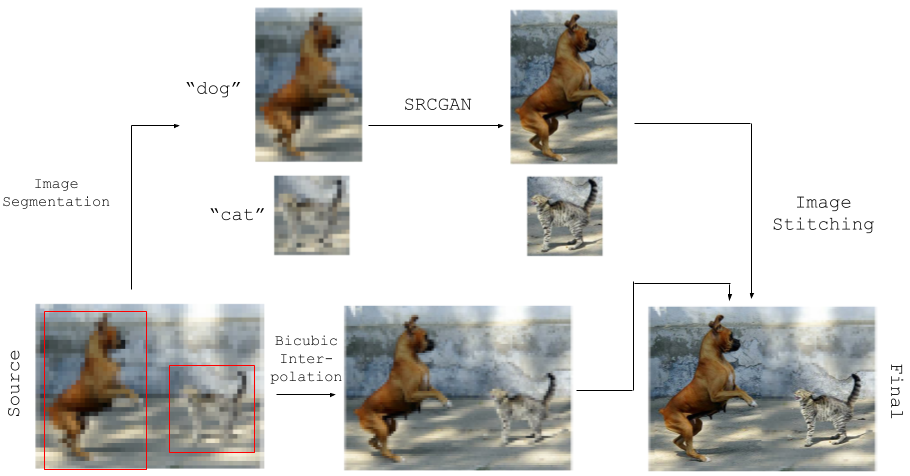
\includegraphics{images/intuition.png}
	\caption{An example of how our technique would work end-to-end. The source
	image (bottom right) would first be put through an Image Segmentation
	algorithm to determine the different subjects in the image. Once the subjects
	and their classes have been determined, they are then run through the SRCGAN.
	In the meanwhile, the whole image is run through a bicubic interpolation. Once
	the higher quality images have been formed, they are merged together through
	the image stitching algorithm. Once the images have been stitched together,
	the final image will be formed.}
	\label{fig:intuition}
\end{figure}

This process is illustrated by Figure \ref{fig:intuition}. By breaking the process up into smaller, more manageable chunks, one is able to take advantages of the different top-performing models. The following sections will go into greater detail on the reasons behind choosing the various methods and how they were implemented.

\subsection{Dataset Selection}

We opted to select datasets with one to three subjects in it in order present
where our proposed solution would shine. The datasets we selected for training
were created by splitting open source HD footage frame by frame. This allowed us
to create large easy to label datasets with ease.

\subsection{Segmentation}
\subsubsection*{Fully Convolutional Network}

Fully Convolutional Network (FCN) is one of the states of the art techniques for
semantic segmentation. Semantic segmentation \cite{Liu2018} refers to the process of
associating each pixel in an image with a class label such as animals, roads,
buildings, etc. FCNs build up on CNN. CNNs are very good for image
classification data but they do not retain any spacial information with
convolutions. All the features are detected but their locations in the image are
not maintained. FCNs improve on this by just having convolutional layers. A
typical FCN network consists of an encoder block, 1x1 convolutional layer,
decoder block. The encoder block is pretty much the same as a CNN without the
fully connected layers. It downsamples the image with each convolution and
increases the feature maps. 1x1 convolutions are used to change the filter
dimensionality (either increase it or decrease it) before sending it to the
decoder block. The decoder block consists of transposed convolutional layers
often called deconvolutional layers. This part of the network deals with
upsampling the image to its original size. The output at the end is a image
associating each pixel with a class.

\begin{figure}
	\centering
	
	\begin{subfigure}[h]{0.4\textwidth}
		\centering
		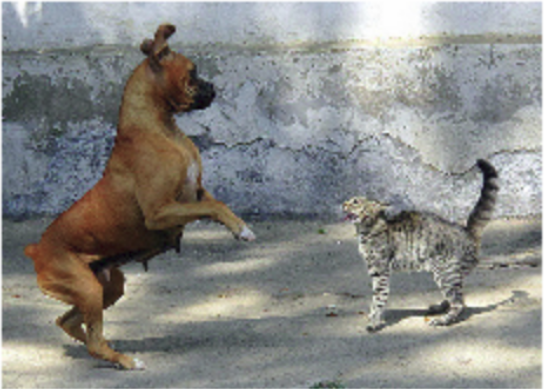
\includegraphics[width=\textwidth]{images/fcn-before.png}
		\caption{The source image fed into Google's DeepLab FCN.}
		\label{fig:fcn-before}
	\end{subfigure}

	\begin{subfigure}[h]{0.4\textwidth}
		\centering
		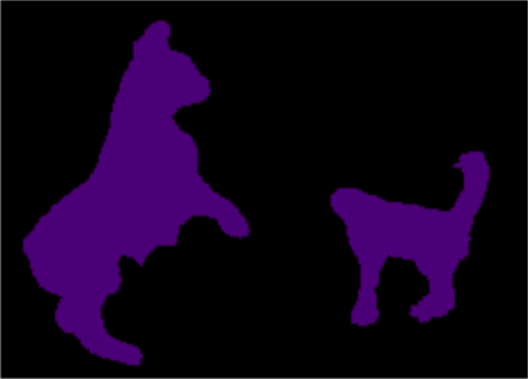
\includegraphics[width=\textwidth]{images/fcn-segmap.png}
		\caption{FCN's classification results. All of the subjects of interest are
		in purple, while the background is black.}
		\label{fig:fcn-segmap}
	\end{subfigure}

	\begin{subfigure}[h]{0.4\textwidth}
		\centering
		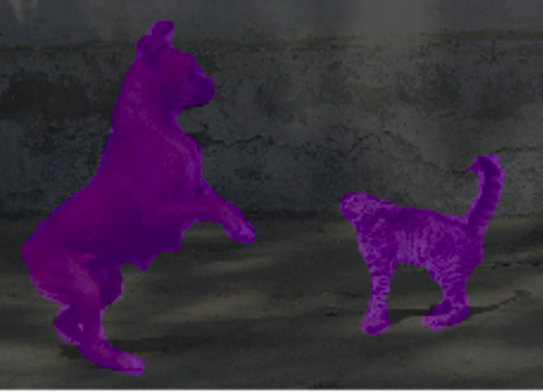
\includegraphics[width=\textwidth]{images/fcn-overlay.png}
		\caption{The FCN results overlayed on the original image.}
		\label{fig:fcn-overlay}
	\end{subfigure}

	\caption{Google's DeepLab Fully Convolutional Network.}
	\label{fig:fcn}
\end{figure}

We decided to use Google’s pre-trained DeepLab FCN \cite{Chen2017}. It is able to perform
this network to get a semantic segmentation output for the backgrounds and
object of interest. These objects of interest are then cropped out as individual
images to be fed into the super-resolution algorithm. The intact background is
passed forwards as well to the further methods.

\subsection{Super Resolution}
\subsubsection{General Adversarial Networks}
General Adversarial Networks (GANs) were first introduced by Goodfellow et al.
in 2014 \cite{Goodfellow2014}. GANs were a new framework that trained generative
models using an adversarial process. Under this framework, there are two models:
a generative model $G$, which trains off of the data distribution, and a
discriminative model $D$, which determines whether a sample is real or has been
generated. Both of the models are trained simultaneously, resulting in a
two-player game of sorts. In this game, $G$ generates a sample and $D$ tries to
guess whether or not the sample is real or not. In order to beat $D$, $G$ has to
create samples that are closer to the data set. Conversely, in order to beat $G$,
$D$ has to become more selective on what is a truth or not. This back and forth
process can intuitively be expressed as a generic 2-player minmax game:

\begin{IEEEeqnarray}{rCl}
	\min_{G}\max_{D}(D, G) = \nonumber\\
	E_{x p_{data}}[\log(D(x))] + E_{z p_{z}(z)}[\log(1 - D(G(z)))]
\end{IEEEeqnarray}

\subsubsection{Conditional GANs}
Mirza and Osindero improved upon Goodfellow et al.’s vanilla GAN by simply
adding auxiliary features to inputted data \cite{Mirza2014}. These “conditioning
features” are added as inputs to both the discriminator and generator functions
as well as labels to the data. These modifications can be seen in the following
objective function:

\begin{IEEEeqnarray}{rCl}
	\min_G\max_D(D,G) = E_{x p_{data}}[\log(D(x|\mathbf{y}))] \nonumber\\
	+ E_{z p_z(z)}[\log(1 - D(G(z|\mathbf{y})))]
\end{IEEEeqnarray}

In which the auxiliary feature vector is represented by $\mathbf{y}$. \\

Mirza and Osindero were able to successfully generated MNIST digits conditioned
on both the MNIST dataset and the respective class labels. \cite{Mirza2014} \\


\subsubsection{Super Resolution with CGANs}
GANs are currently some of the top methods for super resolution and CGANs have
been shown to work well in combining GANs and auxiliary information. Chen et al.
combined the two ideas by using CGANs for image super resolution \cite{Chen}. In
their report, Chen et al. introduce two methods of introducing new features into
their Super Resolution GAN (SRGAN)\cite{Chen}:

\begin{enumerate}
	\item (SRCGAN) - Add the class information as another input feature.
	\item (SRGAN + Class Loss) - Create an independant classifier whose purpose is
		to determine if the generated image is of the correct class and factor that
		into the objective function.
\end{enumerate}

In this project, an SRCGAN was chosen due to its demonstrated accuracy
improvements over a vanilla GAN \cite{Chen}. As per Chen et Al.’s findings, the
objective function for this model is as follows:

\begin{IEEEeqnarray}{rCl}
	\min_{\Theta_G}\max_{\Theta_D}(D, G) = \nonumber\\
	E_{I^{HR}\sim p_{train}}(I^{HR})[\log(D_{\Theta_D}(I^{HR}, \mathbf{c}))] \nonumber\\
	+ E_{I^{LR}\sim p_G(I^{LR})}[\log(1 - D_{\Theta_G}(G_{\Theta_G}(I^{LR},
		\mathbf{c})), \mathbf{c})]
\end{IEEEeqnarray}

In which $\mathbf{c}$ is the conditional information, $D$ and $G$ are the
updated discriminator and generator functions, and $I^{HR}$ and $I^{LR}$ are the
high-resolution and low-resolution images, respectively.

For the creation of the SRCGAN, Linder-Norén’s implementation of the SRGAN
\cite{Linder-Noren} from Ledig et Al  was used as a bootstrap due to its success in
photo-realistic super resolution \cite{Ledig}. The class information of the sample
subject was then added as another feature to the input vector and the objective
function was modified to account for the change in the feature space.

While Chen et Al. discuss that using class data as auxillary inputs in the
SRCGAN is trivial, they were only working on the MNIST and CelebA datasets
\cite{Chen}. In this case, it is trivial to see how class information (such as
“person”) would be a trivial feature to add, as all of the samples would share
the same information \cite{Chen}. However, this application hosts a variety of
different classes for subjects to be in, so including the class information
plays a non-trivial role. \\

\subsubsection{Bicubic Interpolation}
While GANs have made impressive advances in image super resolution, they are not
without fault. As Goodfellow discusses \cite{Goodfellow2017}, GANs tend to have
issues when dealing with:

\begin{itemize}
	\item Counting
	\item Perspective
	\item Global Structures
\end{itemize}

While these drawbacks may be a bit more trivial when working on more restrictive
datasets such as MNIST or CelebA, they become more of an ordeal when dealing
with complex, multi-subject images. For that reason, the SR model chosen for the
base images was Lukin et al.’s Bicubic Interpolation SR model from 2006
\cite{Lukin2006}. The Bicubic Interpolation SR model has seen impressive results in a scaling
factor of 2x and is now considered a baseline SR model. For this project,
OpenCV’s bicubic interpolation implementation was used \cite{Bradski2000}.

\subsection{Image Stitching}
One side-effect of the processes described in this paper is that the subjects of
the image and the background are separated. As a result, the images need to be
stitched back together into one final product image. Python’s OpenCV library and
PIL (Python Imaging Library) are utilized to accomplish this task. Provided the
(x,y) coordinate and (width, height) of the extracted subject image from the
original image, PIL inserts the new subject images back into the main image at
their original locations. The data for this operation is retrieved during the
image segmentation process.

However, a simple copy/paste procedure wouldn’t be enough to truly recreate an
image. Since the background image and the subject images have different
resolutions, the combined image has the possibility of looking somewhat awkward
on the edge of the background and subject image from the sudden change in
resolution. OpenCV has functionality that can be implemented to blur parts of an
image with a certain intensity, which is used here to blur along the shared
edges with different intensity such that the transition from the background
image to subject image looks more natural.


% Results
\section{Results}
\subsection{Overview}
In theory, this project is designed to overcome the shortcomings of different
methods in order to have a more optimal outcome. To reiterate, the primary
shortcomings of current methods in relation to complex (multi-subject images)
are:

\begin{itemize}
	\item Bicubic Interpolation \& Non Deep Learning approaches - generally have
been to be found less effective than DL solutions
	\item GANs (and other DL approaches) - are known to have problems with
counting, perspective, and global structures. It is theorized that these
problems could be overcome with a more complex model architecture, but we do not
have the hardware to properly test that \cite{Goodfellow2017}.
\end{itemize}

By segmenting the subjects of the images out, this method effectively minimizes both drawbacks. Segmenting the images gets rid of the counting, perspective, and global structures issues for GANs. Additionally, because GANs are known to produce better results than bicubic interpolation, having the subjects of interest be enhanced by GANs will produce a stronger image overall.

Our team had two main issues in the execution of this project:

\begin{enumerate}
	\item We didn’t have the hardware to train all of the models from scratch, so
we tried to use as many “off the shelf parts” as possible.
	\item We tried to parallelize the development of this project as much as possible. 
\end{enumerate}

While these methods work for working on each component in seclusion, they are
unoptimized for creating the final end-to-end solution. As of the time of
writing this paper, we have different parts of this technique working, but
currently, don’t have any results for the combined model. \\

These results will be available in the final revision of this report.

\subsection{Super Resolution}

\begin{figure}
	\centering
	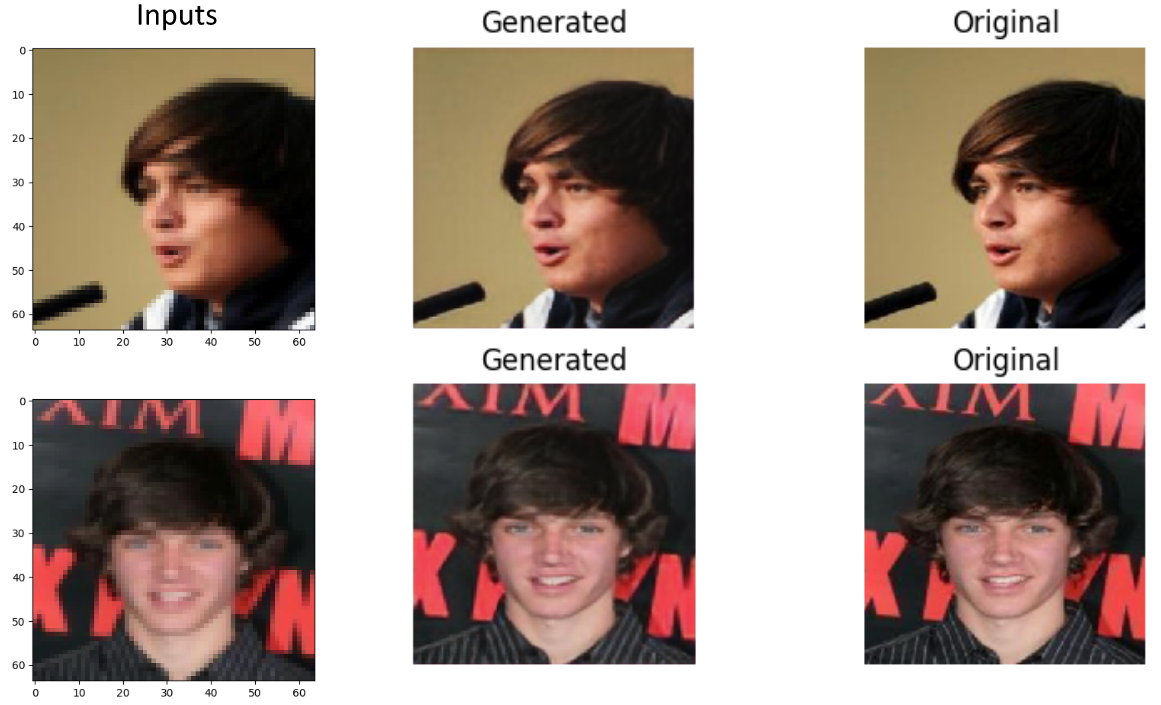
\includegraphics[width=0.45\textwidth]{images/gan-res.png}
	\caption{Results of the SRCGAN when run on the CelebA dataset after 6900
	iterations. The images on the left are the inputted images, alongside class
	information, the images in the middle are generated images, and the image on
	the right are the ground truth}
	\label{fig:gan-res}
\end{figure}

The results for the SRCGAN are shown in \ref{fig:gan-res}. The specific model was
trained for 6900 iterations. As shown in the figure, the GANs tends to perform
well in creating an image which has similar semantics to the ground truth. In
fact, if one didn’t know about the existence of the ground truth, it is entirely
possible to believe that the generated image isn’t fake.

PSNR is what is planned to be used in the measuring the final performance of the
super-resolution algorithm. Unfortunately, at the time of writing this paper,
the technique wasn’t in a state to present the PSNR results. These results will
be available in the final iteration of this paper.

\subsection{Stitching}
Before undergoing image stitching, the subject images and background image are
all separated as individual images. An example of this separation is shown
below:

[BACKGROUND IMAGE]
[SUBJECT IMAGE X] [SUBJECT IMAGE X] [SUBJECT IMAGE X] ...

From here, PIL is used to take the subject images and place them in their
appropriate places on the background image. Their positions are determined from
data provided by the image segmentation algorithm that gives the (x,y)
coordinate of the specified subject image in the background image and the
original subject image’s height and width dimensions. This reconstruction
results in a single image, an example of which is demonstrated below:

[RECONSTRUCTED IMAGE]

Now that all the images are merged into one image, blurring along the shared
edges between the subject images and background image needs to be done to make
the entirety of the image look more natural. This is done using OpenCV’s image
blurring functionality with a blur radius of (WIDTH, HEIGHT). The blurring is
done in such a way as to make a smooth transition from the resolution of the
subject images to the resolution of the background image. An example of the
final product can be seen below:

[IMAGE]

More details about the results of the image stitching process will be available
in the final iteration of this paper.


% Conclusion
\section{Conclusion}

In theory, with our method we achieve the best of both worlds: having access to the power of SRCGAN’s for the more important parts of the images we superresolution while saving on computation costs by not training on as much noise. However, due to not having the hardware to train an FCN and using third party libraries, our current end product has to re-calculate various values.
Our method is also restricted by the limitations of SRCGAN’s. Since SRCGAN’s
have a fixed nxn sized input, we have to either upscale or downscale our FCN
output in order to pass it to the SRCGAN. Additionally, when we have long or
tall subjects, like a giraffe, we need to pass additional background information
that we know isn’t our subject into the SRCGAN (as seen in Figure \ref{fig:giraffe}), resulting in
noise when both training and running the SRCGAN.

\begin{figure}
    \centering
    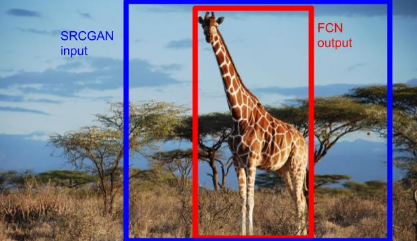
\includegraphics[width=0.45\textwidth]{images/giraffe.png}
    \caption{An example of an inefficiency with our method. Although the FCN knows the giraffe is bounded within the red box, due to the nature of SRCGAN's we are forced to pass the blue box, essentially wasting computation.}
    \label{fig:giraffe}
\end{figure}


Another issue with our method is when multiple subjects overlap. Since we run our SRCGAN for each image we classify, any overlap is enhanced multiple times, causing unnecessary calculation as seen in Figure \ref{fig:crossover}. As such, our method would not work well when the FCN classifiers more area as subjects than the size of the original image.

\begin{figure}
    \centering
    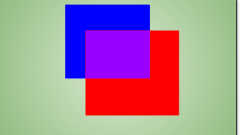
\includegraphics[width=0.45\textwidth]{images/crossover.png}
    \caption{If the FCN classifies the red area as one class and the blue are as another, the purple area is run through the SRCGAN twice.}
    \label{fig:crossover}
\end{figure}


\section{Future Work}

Our goal for Context Aware Super Resolution is to one day use it for video compression. The end goal would be to have . While current research has shown potential for video compression using super resolution, nothing pratical has yet to be created [1][2]. We hope to create a refined version of our method that could potentially be used for compression videos with a low subject count (Figure \ref{fig:compression})


\begin{figure}
    \centering
    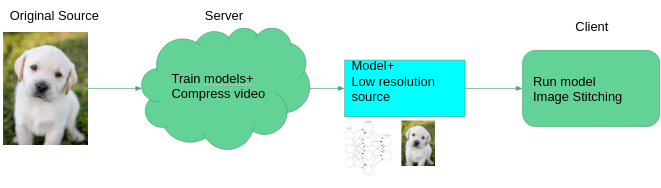
\includegraphics[width=1\textwidth]{images/compression.png}
    \caption{A potential server-client model for video compression using Context Aware Super Resolution}
    \label{fig:compression}
\end{figure}



% use section* for acknowledgment
\ifCLASSOPTIONcompsoc
  % The Computer Society usually uses the plural form
  \section*{Acknowledgments}
\else
  % regular IEEE prefers the singular form
  \section*{Acknowledgment}
\fi


The authors would like to thank...


% trigger a \newpage just before the given reference
% number - used to balance the columns on the last page
% adjust value as needed - may need to be readjusted if
% the document is modified later
%\IEEEtriggeratref{8}
% The "triggered" command can be changed if desired:
%\IEEEtriggercmd{\enlargethispage{-5in}}

% references section

% can use a bibliography generated by BibTeX as a .bbl file
% BibTeX documentation can be easily obtained at:
% http://mirror.ctan.org/biblio/bibtex/contrib/doc/
% The IEEEtran BibTeX style support page is at:
% http://www.michaelshell.org/tex/ieeetran/bibtex/
%\bibliographystyle{IEEEtran}
% argument is your BibTeX string definitions and bibliography database(s)
%\bibliography{IEEEabrv,../bib/paper}
%
% <OR> manually copy in the resultant .bbl file
% set second argument of \begin to the number of references
% (used to reserve space for the reference number labels box)

% \begin{thebibliography}{1}
% 
% \end{thebibliography}

% that's all folks
\end{document}
